\documentclass{llncs}
\usepackage[T1]{fontenc}
\usepackage{graphicx}
\usepackage{amsmath}
\usepackage{listings}
\usepackage{tikz}
\usepackage{epstopdf}
\usepackage{multirow}
\usepackage{todonotes}

\title{Evaluating the Effectiveness of AEX-Notify against SGX Single-Stepping Attackers}
\author{Wicked Wench}
\institute{	University of L\"ubeck, Germany}
% TODO: For the camera-ready submission
%\author{Basil Ugbomoiko\inst{1} \quad Daniel Knaack\inst{1}}
%\institute{	University of L\"ubeck, Germany\\
%	\email{\{basil.ugbomoiko,daniel.knaack\}@student.uni-luebeck.de}}

\begin{document}

\maketitle

%\begin{abstract}
%A short description of your project (150-250 words).
%
%This document is intended as a guide to structure your project and to help you
%to document your work in a paper structure.
%\end{abstract}


\section{Introduction}

\paragraph{Background on SGX-Step attacks}
\begin{itemize}
  \item Explanation of SGX Technology 
  \item Brief overview of SGX-Step attacks and their implications
\end{itemize}

\paragraph{Introduction to AEX-Notify}
\begin{itemize}
  \item Overview of AEX-Notify
  \item Potential benefits of using AEX-Notify
\end{itemize}

\paragraph{Research Question and Objectives}
\begin{itemize}
  \item Formulation of the \textbf{research question}:
    Is it possible to gather control-flow information of victim programs running
    in SGX enclaves when the victim protects the execution of the enclave with
    AEX-Notify?
  \item \textbf{Project goals}:
    Our goal is to evaluate the effectiveness of AEX-Notify against SGX-step by
    constructing an example program where the SGX-Step attack works and testing
    this program once with AEX-Notify enabled and once without. We will compare
    the results to see how much information we can gain about control-flow
    information with and without AEX-Notify enabled.
\end{itemize}

\section{Related Work}
\begin{itemize}
  \item 
    Look into the necessary background for the three main mechanisms
    behind this project: SGX-Step, CopyCat and AEX-Notify.
\end{itemize}

\subsection{SGX-Step} 
\begin{itemize}
  \item Interrupt SGX enclave using APIC timer.
  \item Problem: Finding the correct time interval to resume right after \texttt{ERESUME} instruction.
    \begin{itemize}
      \item Arriving too early would resume within the \texttt{ERESUME} instruction would result in zero-step.
      \item Arriving too late would execute more than one instructions.
    \end{itemize}
  \item Previous methods configured the timer in kernel space, resulting in large time jitter.
  \item APIC timer is configured in user space.
\end{itemize}

\subsection{CopyCat}
\begin{itemize}
  \item uses SGX-Step to track intra-page control-flow of an enclave application.
  \item infers the branch that was taken from data access patterns. See switch example.
\end{itemize}

\subsection{AEX-Notify}
\begin{itemize}
  \item Mechanism of action: How does it mitigate the SGX-Step attack?
  \item Previous studies on AEX-Notify
\end{itemize}

\begin{figure}[t]
  \centering
  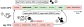
\includegraphics{images/sgx-step-pte.pdf}
  \caption{\todo[inline]{Add a proper caption here.}}
  \label{fig:sgx-step-pte}
\end{figure}

The main reason behind the effectiveness of the SGX-Step attack is the assisted
page-table walk.
Before resuming the enclave, the SGX-Step framework will clear the present bit
on the pages, which causes a page fault when executing the first instruction.
This induces additional latency in the execution of the instruction, because
the processor has to walk the page table again.
Thus, there is a large time frame where the interrupt of the timer could
arrive and land exactly on the first instruction.
The goal of AEX-Notify is to reduce the latency of the first instruction
and make it impossible to land exactly on the first instruction.

\todo{Explain how the instruction works.}
\todo{Explain the AEX-Notify interrupt mechanism.}
The first step is an ISA extension that introduces a new instruction \texttt{EDECCSSA}.

AEX-Notify does not work on its own.
Instead, it provides the means necessary to implement a mitigation in software.

\paragraph{Software Mitigation}
The goal of the mitigation is to reduce the latency of the first instruction.
In order to achieve this, it is important that the first instruction never causes any page faults.
Otherwise, we would need to walk the page table again increasing the latency of the instruction.
Thus, our software mitigation implements a prefetcher.
This prefetcher will always fetch necessary code and data pages of the resumed
instruction which ensures that no faults can occur.

With the software mitigation enabled, an interrupt can arrive at three possible
locations during the execution.
First, it could arrive too early and land in our prefetching code.
This would not cause any problems as resuming the enclave a second time would
call the prefetcher again and would load the same pages as before.
Next, the interrupt could arrive to late and land after the first instruction.
In this case, we would have executed more than one instruction which means
that we have successfully avoided single-stepping.
Last, it could arrive perfectly on the first instruction.
This is the exact case that we are trying to avoid.
However, since the code and data pages for this instruction have already been prefetched,
it is unlikely that an interrupt would arrive exactly on the first instruction.
  
\section{Methodology}

\subsection{Single-stepping attack implementation}
\begin{itemize}
  \item Introduction to Zigzagger attack methods
  \item Step-by-step implementation guide
  \item Code snippets and explanations
\end{itemize}

\subsection{Experimental Setup}
\begin{itemize}
  \item Hardware and Software specifications
  \item Configuration details
\end{itemize}

\subsection{Implementation details for applying AEX-Notify}
\begin{itemize}
  \item How AEX-Notify is integrated into the experimental setup
  \item Configuration and setup details
\end{itemize}

%\section{AEX-Notify Countermeasure}

%\begin{itemize}
%  \item Description of how AEX-Notify works
%  \item Implementation details for applying AEX-Notify to protect the enclave
%  \item Results comparing enclave execution with and without AEX-Notify
%\end{itemize}

\section{Evaluation and Results}
\subsection{Analysis of Single-stepping attack results}
\begin{itemize}
    \item Observations and findings
\end{itemize}
\subsection{AEX-Notify Countermeasure}
\begin{itemize}
    \item Performance metrics with AEX-Notify
    \item Comparative analysis of enclave execution
\end{itemize}

\section{Discussion}
\begin{itemize}
  \item Discussion of findings and interpretation of results
  \item Implications for SGX security
  \item Limitations of the study and challenges faced during the study
\end{itemize}

\section{Conclusion and Future Work}
\begin{itemize}
    \item Summary of key findings
    \item Potential enhancements to AEX-Notify
    \item Future research directions
\end{itemize}

\bibliographystyle{alpha}
%\bibliographystyle{splncs03}
\bibliography{references}
\end{document}
